\documentclass{standalone}
\begin{document}
	\subsection{Expert Evaluation}
	
	An other measure fo the quality of the segmentation was a blind evaluation, in which the achieved segmentation was compared to a reference one. As a reference we have usedthe labels given by the public dataset and the segmentation made by Sant'Orsola internals. 
	
	To perform the evaluation  we have randomly select $40$ patients from the three dataset and organized the scans as follows:
	For each patient we have displayed, slice by slice,  two images: the scans with the pipeline segmentation(the one to test), and the manual labels provided within the dataset (control) as in \figurename\,\ref{fig:Blind}.
	
	\begin{figure}[h!]
		\centering
			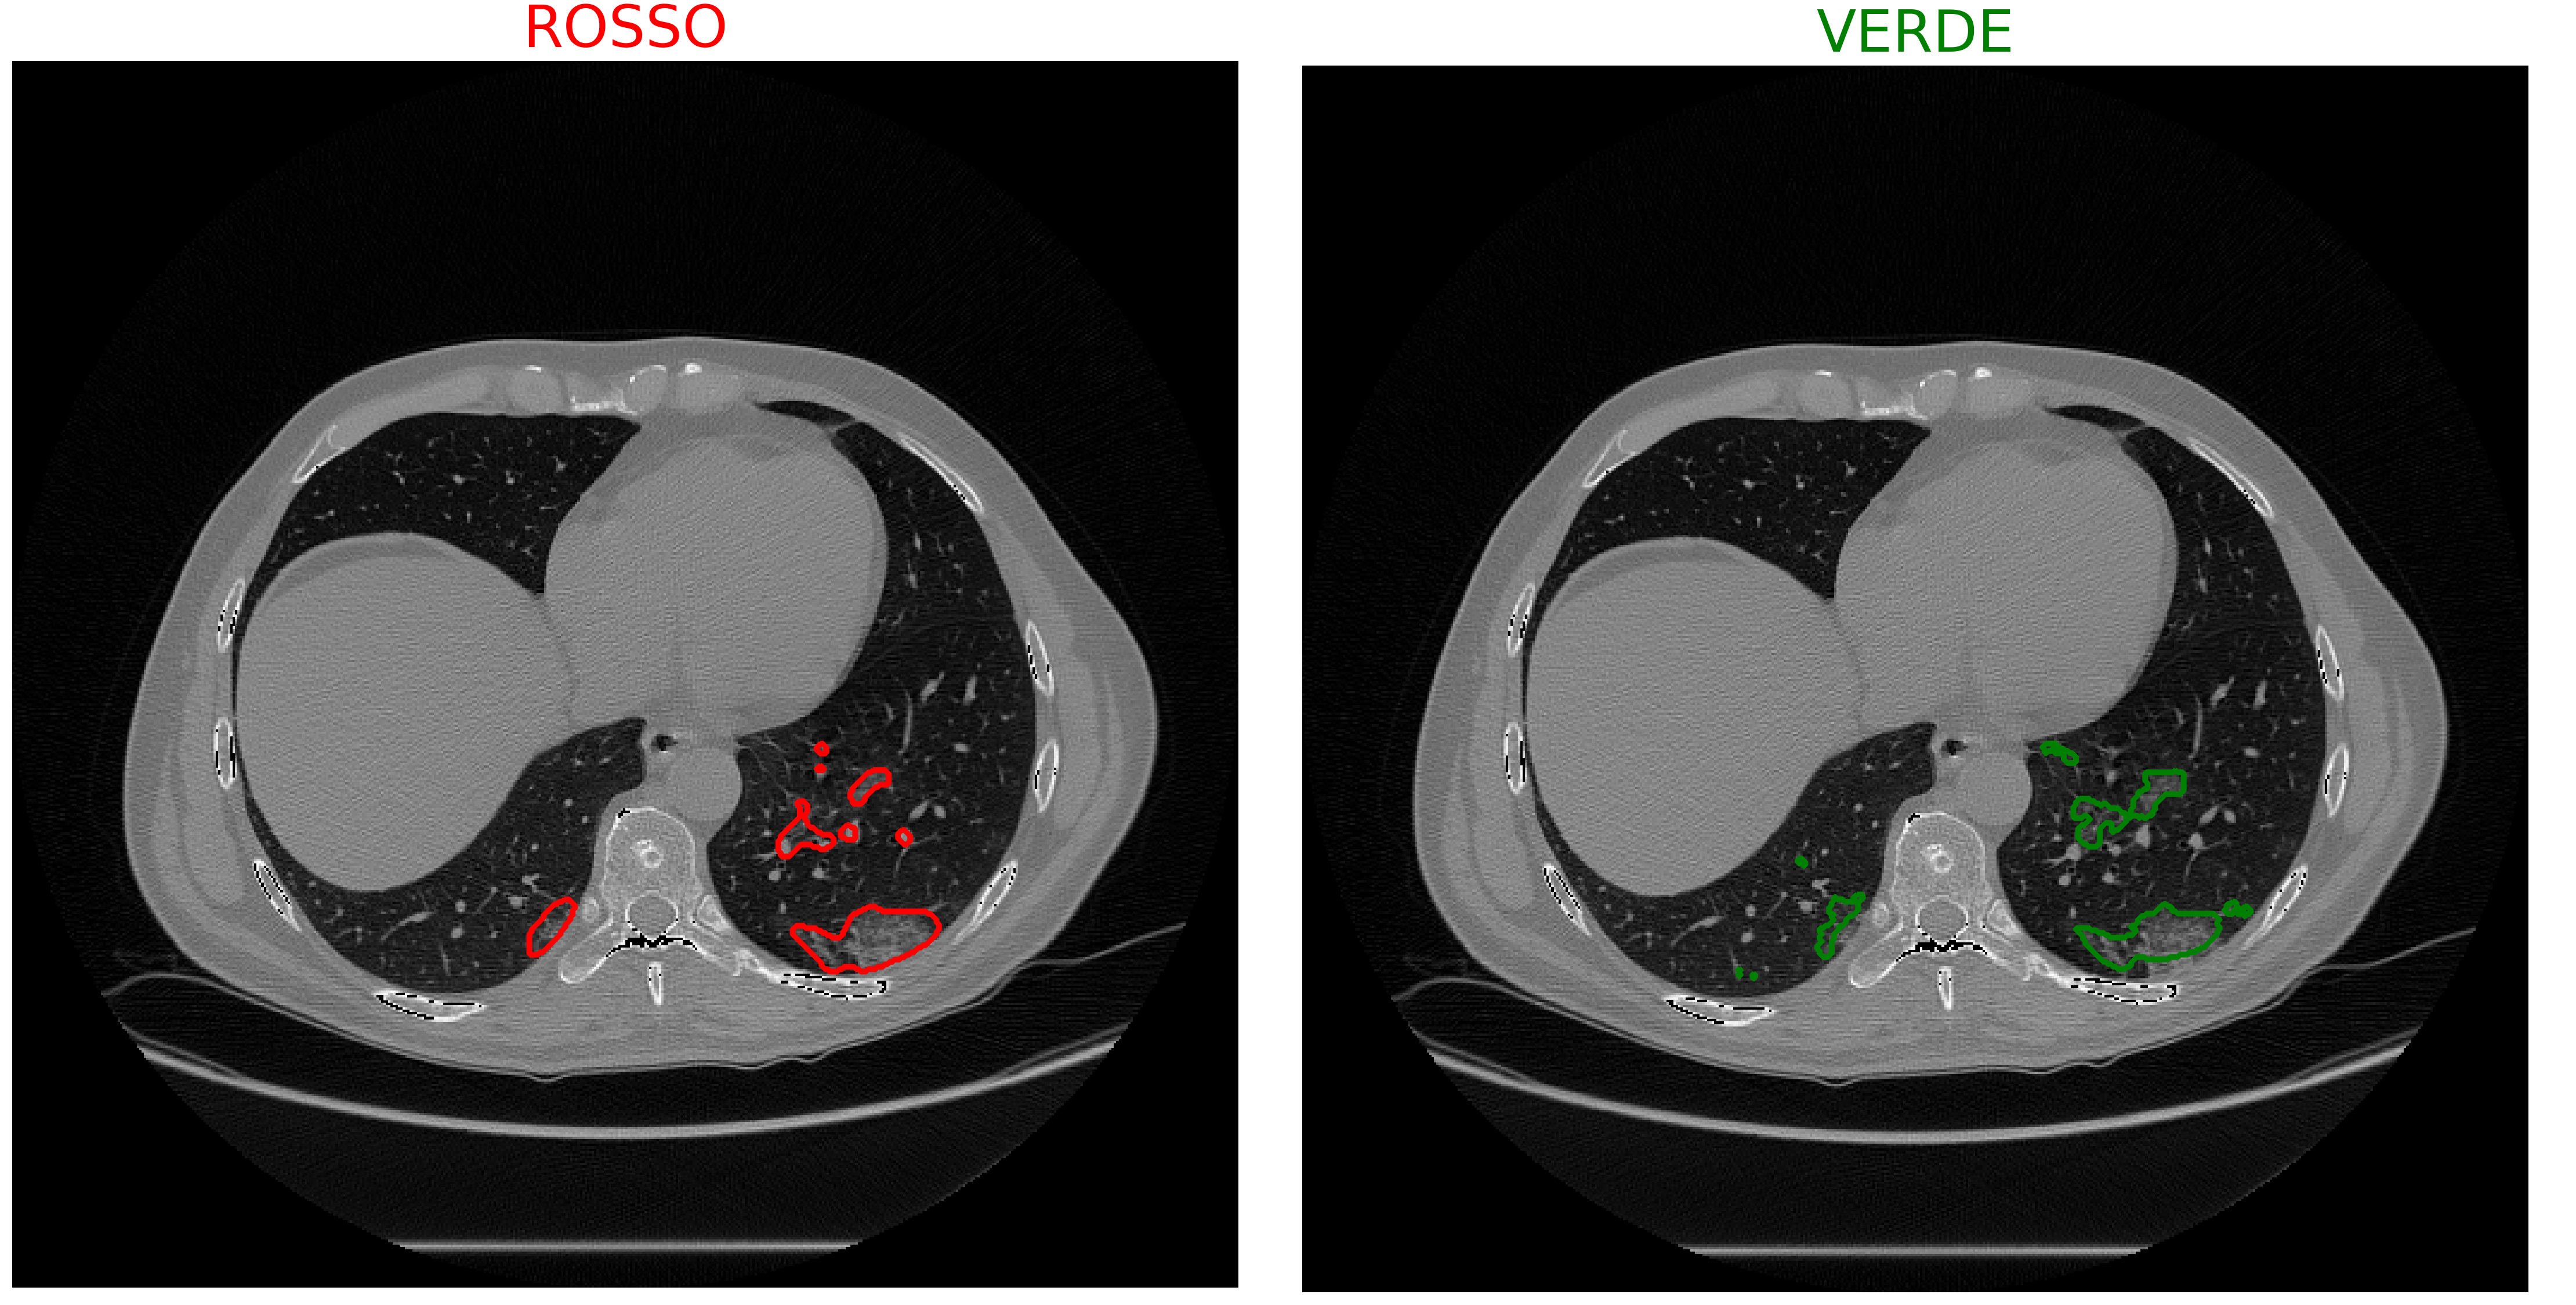
\includegraphics[scale=.3]{BlindEval.png}
			\caption{Example of comparison submitted to the experts. The two images report the segmentation of the same slices achieved with two different techniques: Manual and pipeline. Was asked to the expert to decide which one is better, without knowing which technique is used to obtain the segmentation.}\label{fig:Blind}
	\end{figure}

	The scans, organized in this way, was evaluated by experts, to which has been asked to decide, slice by slice, which segmentation is better or if the quality is equal.
	
	The core of this method is that the expert doesn't know which scan correspond to a specific segmentation technique, so this will lead to an ideally unbiased evaluation.  In order to ensure that, the order of segmentation was shuffled between patients. 
	
	

	
\end{document}